% Created 2020-03-23 Mon 23:14
% Intended LaTeX compiler: pdflatex
\documentclass[11pt]{article}
\usepackage[utf8]{inputenc}
\usepackage[T1]{fontenc}
\usepackage{graphicx}
\usepackage{grffile}
\usepackage{longtable}
\usepackage{wrapfig}
\usepackage{rotating}
\usepackage[normalem]{ulem}
\usepackage{amsmath}
\usepackage{textcomp}
\usepackage{amssymb}
\usepackage{capt-of}
\usepackage{hyperref}
\author{rraks}
\date{\today}
\title{}
\hypersetup{
 pdfauthor={rraks},
 pdftitle={},
 pdfkeywords={},
 pdfsubject={},
 pdfcreator={Emacs 27.0.90 (Org mode 9.4)}, 
 pdflang={English}}
\begin{document}

\tableofcontents

\section{IUDX Migrating to better linked data}
\label{sec:org8cd3bdb}


\section{Getting started}
\label{sec:org4b8a498}
\subsection{Basic items}
\label{sec:org3b26ea5}
\subsubsection{Following schema.org \href{https://schema.org/}{json-ld form}}
\label{sec:org017acbf}



\subsubsection{Do we use schema.org standard terminologies such as \href{https://schema.org/Thing.jsonld}{``Thing''} instead of ResourceItem?}
\label{sec:org4d130c9}
\begin{enumerate}
\item JSON
\label{sec:orgbe4459f}
\begin{verbatim}
{
    "@context": {
        "schema": "http://schema.org/"
    },
    "@graph": [
        {
            "@id": "schema:dataFeedElement",
            "schema:rangeIncludes": {
                "@id": "schema:Thing"
            }
        },
        {
            "@id": "schema:name",
            "schema:domainIncludes": {
                "@id": "schema:Thing"
            }
        }
    ]
}
\end{verbatim}
\item LD Expansion
\label{sec:org1c189cb}
\begin{center}
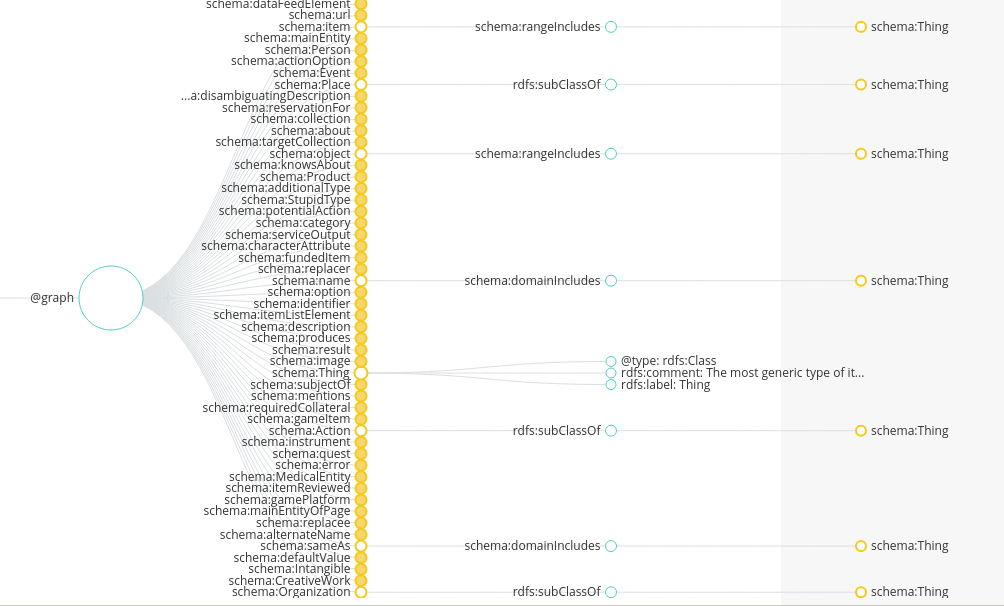
\includegraphics[width=.9\linewidth]{./graph.png}
\end{center}
\end{enumerate}


\subsection{Basic Types}
\label{sec:org57043eb}
\subsubsection{schema:measuredValue is essentially iudx:QuantitativeProperty}
\label{sec:orga0fb30e}
\subsubsection{Datatypes in schema.org use schema:DataType}
\label{sec:org065f559}
\subsubsection{What this means}
\label{sec:orgf2ca47c}
\begin{enumerate}
\item JSON
\label{sec:org8120d62}
\begin{verbatim}
{
    "@context": {
        "schema": "http://schema.org/"
    },
    "@graph": [
        {
            "@id": "schema:measuredValue",
            "schema:rangeIncludes": {
                "@id": "schema:DataType"
            }
        },
        {
            "@id": "schema:DataType",
            "@type": "rdf:Class",
            "rdf:comment": "The basic data types such as Integers, Strings, etc.",
            "rdf:label": "DataType",
            "rdf:subClassOf": {
                "@id": "rdf:Class"
            }
        },
        {
            "@id": "schema:Number",
            "@type": "schema:DataType"
        }

    ]
}
\end{verbatim}
\begin{center}
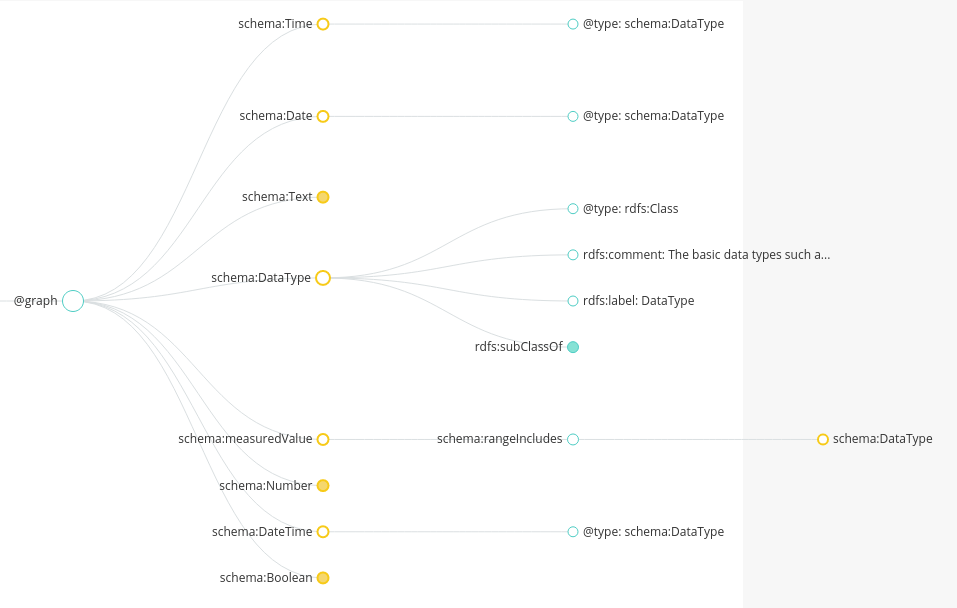
\includegraphics[width=.9\linewidth]{./datatype.png}
\end{center}
\end{enumerate}

\subsubsection{schema.org is flexible is a little ambiguous}
\label{sec:org496e023}
\begin{enumerate}
\item measuredValue doesn't have rdf:subclass or type
\label{sec:orga4a467f}
\item DataType is of @type and subclass off rdf:class\ldots{} why?.. why not rdfs:resource
\label{sec:org39dc05b}
\item Does @type imply rdf:range?
\label{sec:org39f9b62}
\end{enumerate}

\subsubsection{According to this, time is a measured value and therefore, iudx:TimeProperty will be invalidated.}
\label{sec:orgb470604}
\begin{center}
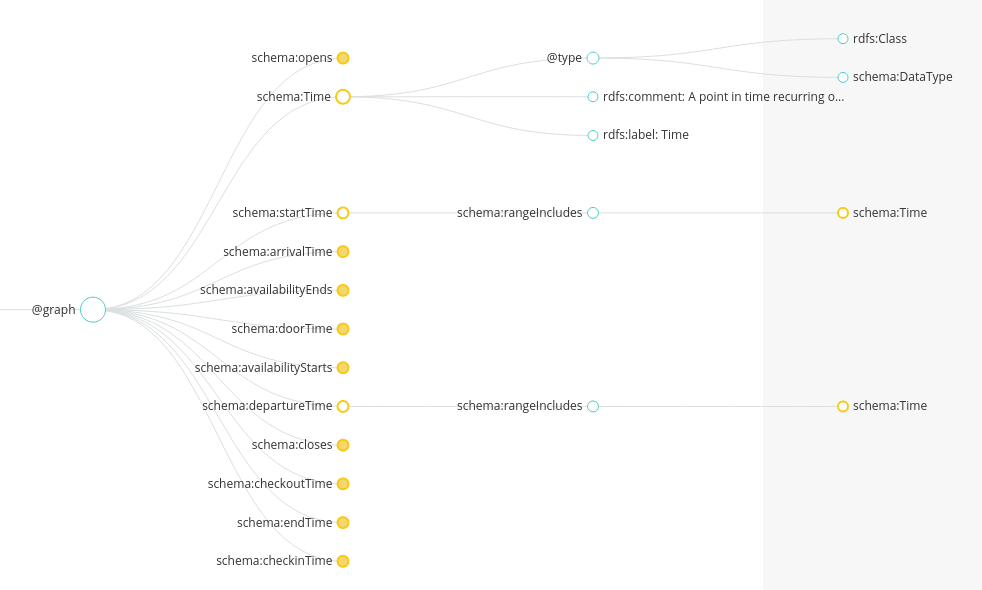
\includegraphics[width=.9\linewidth]{./time.png}
\end{center}

\subsection{A higher level to measuredValue}
\label{sec:org8dc621d}
\subsubsection{Observation - This is what QuantitativeProperty should be. This is in the pending list along with measuredValue}
\label{sec:orgc32b12b}
\begin{verbatim}
[
    {
        "@id": "schema:Observation",
        "@type": "rdf:Class",
        "dcterms:source": {
            "@id": "https://github.com/schemaorg/schemaorg/issues/2291"
        },
        "rdf:comment": "Instances of the class <a class=\"localLink\" href=\"http://schema.org/Observation\">Observation</a> are used to specify observations about an entity (which may or may not be an instance of a <a class=\"localLink\" href=\"http://schema.org/StatisticalPopulation\">StatisticalPopulation</a>), at a particular time. The principal properties of an <a class=\"localLink\" href=\"http://schema.org/Observation\">Observation</a> are <a class=\"localLink\" href=\"http://schema.org/observedNode\">observedNode</a>, <a class=\"localLink\" href=\"http://schema.org/measuredProperty\">measuredProperty</a>, <a class=\"localLink\" href=\"http://schema.org/measuredValue\">measuredValue</a> (or <a class=\"localLink\" href=\"http://schema.org/median\">median</a>, etc.) and <a class=\"localLink\" href=\"http://schema.org/observationDate\">observationDate</a> (<a class=\"localLink\" href=\"http://schema.org/measuredProperty\">measuredProperty</a> properties can, but need not always, be W3C RDF Data Cube \"measure properties\", as in the <a href=\"https://www.w3.org/TR/vocab-data-cube/#dsd-example\">lifeExpectancy example</a>).\nSee also <a class=\"localLink\" href=\"http://schema.org/StatisticalPopulation\">StatisticalPopulation</a>, and the <a href=\"/docs/data-and-datasets.html\">data and datasets</a> overview for more details.",
        "rdf:label": "Observation",
        "rdf:subClassOf": {
            "@id": "schema:Intangible"
        },
        "schema:category": "issue-2291",
        "schema:isPartOf": {
            "@id": "http://pending.schema.org"
        }
    }
]
\end{verbatim}
\begin{center}
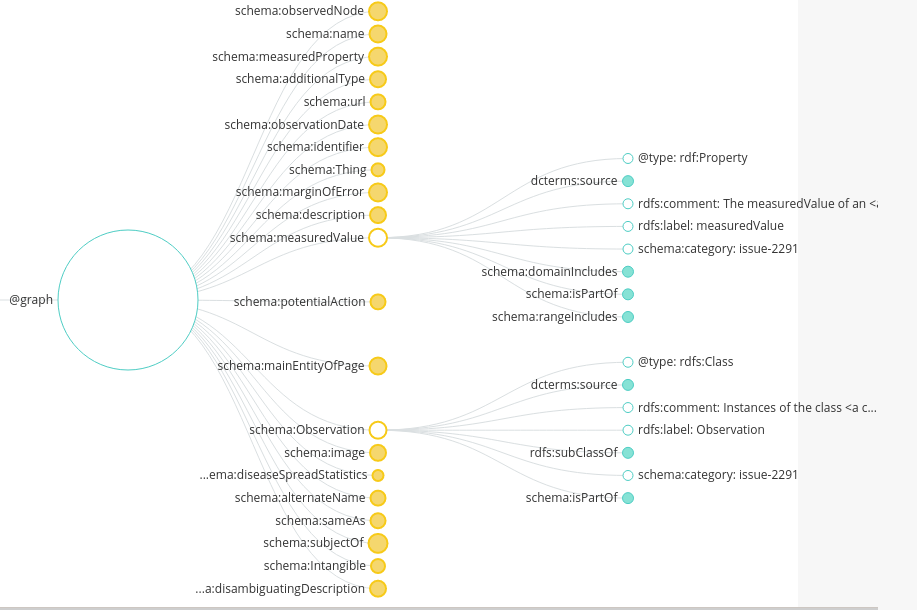
\includegraphics[width=.9\linewidth]{./obs.png}
\end{center}




\section{List of IUDX properties and their mappings}
\label{sec:orgada90e1}

NOTE: schema.org doesn't have rdf:Resource

\subsection{schema.org meta includes - Class, Property, domainIncludes, supersededBy (rangeIncludes??)}
\label{sec:org53bd869}
We need to have our meta (Class, Property) same as schema.orgs'
Basics
\begin{center}
\begin{tabular}{llll}
IUDX & Schema.org & rdf/s & Comments\\
\hline
- & Class & Class & no such definition in iudx\\
- & Property & Class & no such definition in iudx\\
 &  &  & (domain, range) -includes-> Class\\
\hline
- & domainIncludes & Property & no such definition in iudx\\
- & rangeIncludes(Not Present) & Property & \\
\hline
 &  &  & \\
\end{tabular}
\end{center}




IUDX:CoreTypes

\begin{center}
\begin{tabular}{lllll}
IUDX & Schema.org & @type & subClass & Comments\\
\hline
Property & schema:Property & rdfs:Class &  & Generic property describing a thing. Includes relationship\\
 &  &  &  & in schema.org. Shouldn't get confused with rdf:Property,\\
 &  &  & schema:StructuredValue & maybe change name??\\
\hline
QuantitativeProperty & schema:QuantitativeValue & rdfs:Class &  & \\
 &  & or & schema:StructuredValue & \\
 &  & schema:QunatitativeValue &  & \\
\hline
GeoProperty & schema:GeoCoordinates & rdfs:Class & schema:StructuredValue & \\
 &  & or &  & \\
 &  & schema:GeoCoordinates &  & \\
\hline
TimeProperty & schema:Time & rdfs:Class & schema:StructuredValue & \\
 &  & or &  & \\
 &  & schema:Time &  & \\
\end{tabular}
\end{center}

\subsection{We need to differentiate between Observation and QuantitativeValue. All Observations are Quantitative and the reverse is not true}
\label{sec:org6280cf6}
\subsection{schema:StructuredValue seems to be subclass of most of the properties we are intereseted in}
\label{sec:org558e7d4}

\subsection{Example of a few derived attributes}
\label{sec:orga1871a3}
\begin{center}
\begin{tabular}{lllll}
IUDX Property & @type & domainIncludes & rangeIncludes & Comments\\
\hline
name & rdfs:Property & iudx:Property & schema:Text & \\
 &  & and & or & \\
 &  & iudx:ResourceItem & iudx:Text & \\
 &  &  & or & \\
 &  &  & json:String & \\
\hline
lastUpdatedAt & rdfs:Property & iudx:TimeProperty & schema:DateTime & \\
 &  & and &  & \\
 &  & iudx:DataPacket?? & or & \\
 &  &  & iudx:DateTime & \\
 & \\
 &  &  & json:DateTime & \\
\hline
temperature & rdfs:Property & iudx:QuantitativeProperty & schema:measuredValue & Here, we'll need two levels of abstraction\\
 &  &  & or & and talk about measuredValue too. This is because\\
 &  &  & schema:number & a QuantitativeProperty need not be a measuredValue\\
 &  &  & or & \\
 &  &  & iudx:measuredValue & \\
\end{tabular}
\end{center}
\end{document}
